% Authoritative RouterBSI_Draft_Appendix.docx; zero-based direct body paragraph IDs.

% DOCX-P048-BEGIN
\section{Experiments}
% DOCX-P048-END

% DOCX-P049-BEGIN
\subsection{Benchmarks and Skill Corpus.}
% DOCX-P049-END

% DOCX-P050-BEGIN
We conduct experiments on SRA-Bench, which comprises six capability-intensive benchmarks: TheoremQA~\citep{chen-etal-2023-theoremqa}, LogicBench~\citep{parmar-etal-2024-logicbench}, ToolQA~\citep{NEURIPS2023_9cb2a749}, CHAMP~\citep{mao-etal-2024-champ}, MedCalc-Bench~\citep{NEURIPS2024_99e81750}, and BigCodeBench~\citep{ICLR2025_a6a90bcc}. These datasets cover diverse task settings, including mathematical reasoning, formal logic, tool use, and code generation. Each instance is paired with annotated gold skill(s) and evaluated against a shared external skill corpus, enabling decomposed analysis of retrieval, incorporation, and end-task execution. We split each dataset into train, validation, and test splits with ratios of 70\%, 15\%, 15\%, respectively. To evaluate the learning capabilities of baselines, we further filter and balance splits such that each split has at least one task that share the same required skill.
% DOCX-P050-END

% DOCX-P051-BEGIN
\subsection{Evaluation Metrics.}
% DOCX-P051-END

% DOCX-P052-BEGIN
We evaluate skill routing and downstream performance conditioned on the selected skills. For skill routing, we report Recall@\(k\) and nDCG@\(k\). We additionally report F1@\(k\) to compare filtering capabilities. For downstream performance, each benchmark follows its standard evaluation protocol to measure success rate: rule-based exact match or accuracy for reasoning and QA datasets, and pass@1 based on unit-test execution for BigCodeBench. Averages are measured across task instances.
% DOCX-P052-END

% Queue the full-width Results table early; let text fill both columns.
\begin{archivedtables}[!t]% Generated from read-only source CSV.
\begin{table}[!htbp]
\centering
\caption{Skill routing performance on test split across six benchmarks, measured by nDCG@1 (N@1) and nDCG@10 (N@10). Scores are averaged equally across retrievers. Bold and underlined values mark the best and second-best distinct scores in each column. RouterBSI achieves the highest average scores on both metrics.}
\label{tab:skill_routing_performance_average}
\fontsize{8.95pt}{10.8pt}\selectfont
\setlength{\tabcolsep}{1.4pt}
\renewcommand{\arraystretch}{1.06}
\begin{tabular*}{\linewidth}{@{\extracolsep{\fill}}lrrrrrrrrrrrrrr}
\toprule
Method & \multicolumn{2}{c}{\shortstack{BigCode\\Bench}} & \multicolumn{2}{c}{CHAMP} & \multicolumn{2}{c}{LogicBench} & \multicolumn{2}{c}{\shortstack{MedCalc-\\Bench}} & \multicolumn{2}{c}{TheoremQA} & \multicolumn{2}{c}{ToolQA} & \multicolumn{2}{c}{Average} \\
\cmidrule(lr){2-3}
\cmidrule(lr){4-5}
\cmidrule(lr){6-7}
\cmidrule(lr){8-9}
\cmidrule(lr){10-11}
\cmidrule(lr){12-13}
\cmidrule(lr){14-15}
 & N@1 & N@10 & N@1 & N@10 & N@1 & N@10 & N@1 & N@10 & N@1 & N@10 & N@1 & N@10 & N@1 & N@10 \\
\midrule
LLM Select & 0.480 & 0.510 & 0.385 & 0.458 & 0.266 & 0.394 & 0.745 & 0.834 & 0.683 & \underline{0.819} & 0.437 & 0.547 & 0.519 & 0.616 \\
SkillRouter & 0.366 & 0.299 & \underline{0.449} & \underline{0.476} & \underline{0.269} & \underline{0.416} & \textbf{0.974} & \textbf{0.981} & \textbf{0.816} & \textbf{0.860} & \underline{0.600} & \underline{0.711} & \underline{0.619} & \underline{0.671} \\
SkillDAG & \underline{0.612} & \underline{0.600} & 0.359 & 0.453 & 0.143 & 0.378 & 0.709 & 0.785 & 0.651 & 0.781 & 0.161 & 0.421 & 0.429 & 0.576 \\
Skill-Pro & 0.238 & 0.446 & 0.218 & 0.395 & 0.161 & 0.317 & 0.705 & 0.850 & 0.460 & 0.712 & 0.402 & 0.527 & 0.407 & 0.574 \\
$\mathrm{RouterBSI}_{\mathrm{init}}$ & 0.466 & 0.417 & 0.346 & 0.435 & 0.184 & 0.341 & 0.830 & 0.877 & 0.559 & 0.726 & 0.290 & 0.453 & 0.462 & 0.561 \\
RouterBSI & \textbf{0.832} & \textbf{0.707} & \textbf{0.551} & \textbf{0.556} & \textbf{0.336} & \textbf{0.449} & \underline{0.915} & \underline{0.933} & \underline{0.686} & 0.808 & \textbf{0.631} & \textbf{0.712} & \textbf{0.687} & \textbf{0.728} \\
\bottomrule
\end{tabular*}
\end{table}
\end{archivedtables}

% DOCX-P053-BEGIN
\subsection{Selected Models.}
% DOCX-P053-END

% DOCX-P054-BEGIN
We evaluate five models spanning four open-weight checkpoints and one proprietary frontier model: Qwen3.5-4B \citep{qwen2026qwen35}, Qwen3.8-27B \citep{qwen2026qwen38}, Llama-3.3-70B-Instruct \citep{meta2024llama33}, gpt-oss-120b \citep{openai2025gptoss}, and GPT-5.4 \citep{openai2026gpt54}.
% DOCX-P054-END

% DOCX-P055-BEGIN
\subsection{Baselines}
% DOCX-P055-END

% DOCX-P056-BEGIN
We study retrieval, reranker, and selection baselines. The retrievers include sparse and dense retrievers \citep{su2026skillretrieval} and SkillSight, a hybrid retriever. They are trained on training split and frozen on validation and test splits. LLM Select is a static router, and LLM Direct and LLM Oracle are downstream performance baselines representing without skills and with ground-truth skill set, respectively \citep{su2026skillretrieval}. The non-parametric optimization baselines are SkillDag and Skill-Pro \citep{pmlr-v306-mi26d,bai2026skilldag}. $\mathrm{RouterBSI}_{\mathrm{init}}$ and RouterBSI refer to the cold-start and final iteration performance. $\mathrm{RouterBSI}_{\mathrm{strict}}$ selects skills only when their predicate evaluates to true. $\mathrm{RouterBSI}_{\mathrm{top}k}$ are the top k skills using the sum of their predicate label and the retrieval score.
% DOCX-P056-END

% DOCX-P057-BEGIN
\subsection{Implementation Details.}
% DOCX-P057-END

% DOCX-P058-BEGIN
The retrievers use either pretrained embedding models and/or lexical matching, so they do not require training. Candidate skills are retrieved from the shared external skill corpus in response to the input query. The reranking and selection baselines are conditioned on the top 50 retrieved skills and use some optimization method to improve performance. SkillSight is the default retriever for reranking and selection baselines. Qwen3.5-4B is the default model used in our experiments. The non-parametric baselines, including ours, do not output a continuous score like rerankers, so we rank them by the sum of their binary label and the retrieval score, where 1 is the label for selected skills and 0 otherwise. We use a temperature of 1 for proposing candidate predicates and 0 for evaluating predicates and downstream performance. RouterBSI is optimized for 10 iterations. 
% DOCX-P058-END

% Reserve the next page's floats while allowing this page's prose to flow.
\afterpage{%
\begingroup
\let\resultstopfigure\figure
\renewcommand{\figure}[1][]{\resultstopfigure[!ht]}
\begin{figure}[!htbp]
\centering
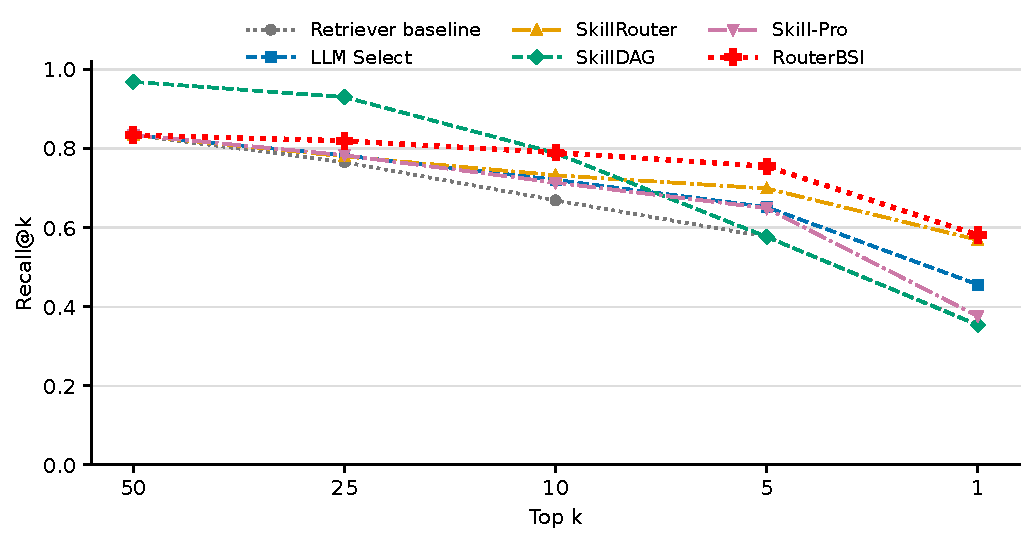
\includegraphics[width=\linewidth]{figs/average_recall_degradation/preview.pdf}
\caption{Required-skill recall comparison as the number of selected skills decreases. Lines show task-weighted test Recall@k averaged equally across BM25, Vector, and SkillSight. The retriever baseline averages the three native retrievers.}
\label{fig:average_recall_degradation}
\end{figure}

\endgroup
% Full-width bottom float; leave the remaining page area for flowing text.
\begingroup
\expandafter\let\expandafter\resultsbottomfigure\csname figure*\endcsname
\expandafter\let\expandafter\endresultsbottomfigure\csname endfigure*\endcsname
\renewenvironment{figure}[1][]{\resultsbottomfigure[!b]}{\endresultsbottomfigure}
% Generated standalone figure; paths are relative to the RouterBSIPaper root.
\begin{figure}[!htbp]
\centering
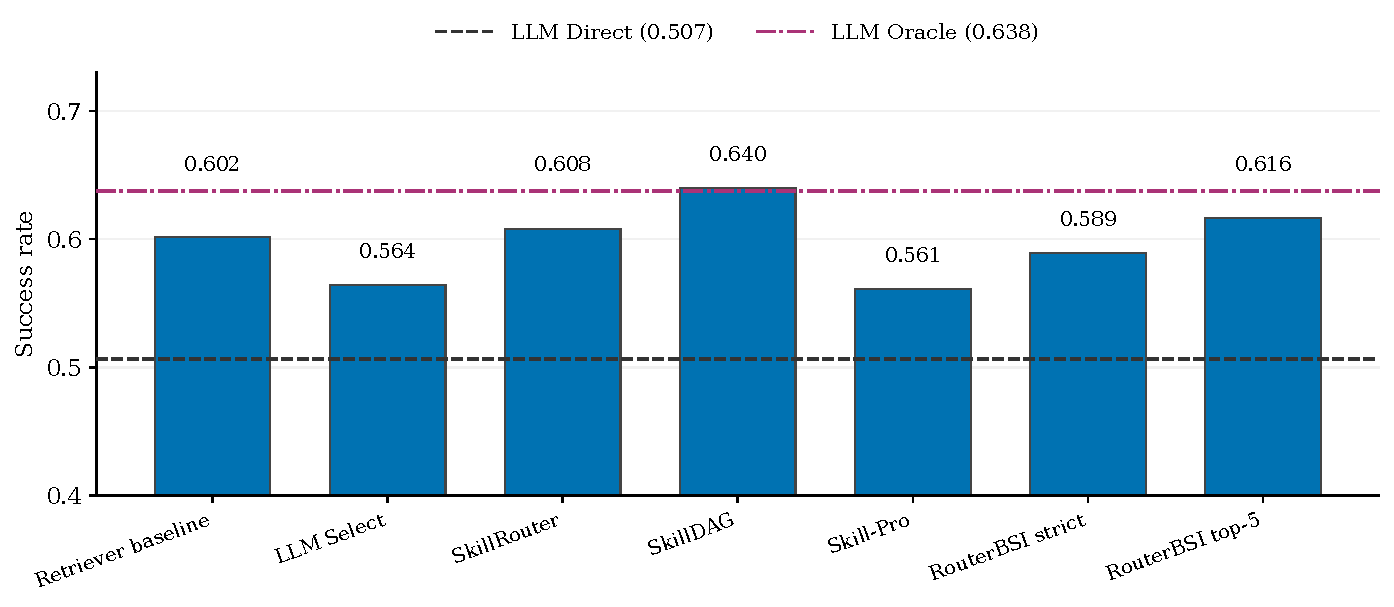
\includegraphics[width=\linewidth]{figs/downstream_average/preview.pdf}
\caption[Downstream average across retrievers]{\input{figs/downstream_average/description.text}}
\label{fig:downstream_average}
\end{figure}

\endgroup
}


